\documentclass[11pt]{article}
\usepackage[margin=1.5in]{geometry}
\usepackage{amsmath}
\usepackage{amssymb}
\usepackage{dsfont}
\usepackage{listings}
\usepackage{graphicx}
\usepackage{float}
\usepackage{booktabs} % Required for professional table lines
\usepackage{xcolor} % Optional, for colored syntax highlighting
\usepackage{tikz} % flow diagram
\usetikzlibrary{arrows.meta}
\usepackage{longtable}
\usepackage{array}
\usepackage{ragged2e}
\usepackage{pdflscape}
\usepackage{xurl}
\usepackage[hidelinks]{hyperref}

\definecolor{dkgreen}{rgb}{0,0.6,0}
\definecolor{gray}{rgb}{0.5,0.5,0.5}
\definecolor{mauve}{rgb}{0.58,0,0.82}
\lstset{frame=tb,
	language=R,
	aboveskip=3mm,
	belowskip=3mm,
	showstringspaces=false,
	columns=flexible,
	basicstyle={\small\ttfamily},
	numbers=none,
	numberstyle=\tiny\color{gray},
	keywordstyle=\color{blue},
	commentstyle=\color{dkgreen},
	stringstyle=\color{mauve},
	breaklines=true,
	breakatwhitespace=true,
	tabsize=3
}

\usepackage[mathscr]{euscript}
\newcommand{\p}{\mathbb{P}}
\newcommand{\e}{\mathbb{E}}
\newcommand{\code}[1]{\nolinkurl{#1}}


\begin{document}

\section{Estimation of the Liquidity-Demand Shock}

Following Telyukova (2013), we use a two-stage empirical procedure to estimate the volatility of innovations in consumer-unit liquid consumption. We then use this empirical moment, together with an adjacent-month consumption-correlation moment, to calibrate the idiosyncratic liquidity-demand shock $\theta_{it}$ in the model. The first-stage specification is

\begin{equation}
	\label{eqn:telyukova_first_stage}
	\log(c^{\mathrm{liq}}_{it})
	= \mathbf{X}_{it}'\beta + \mu_i + \varepsilon_{it},
\end{equation}

where $\mathbf{X}_{it}$ contains a cubic polynomial in age; indicators for education, marital status, race, and homeownership; annual earnings (wage and salary income plus self-employment income); family size; and calendar-month and calendar-year indicators. The term $\mu_i$ is a consumer-unit fixed effect, and $\varepsilon_{it}$ is the idiosyncratic component of log liquid consumption. Although total income before taxes (\lstinline|FINCBTAX|) is retained in the constructed FMLI data, it is not included in the maintained first-stage regression.

In the second stage, we estimate the empirical residual process

\begin{equation}
	\label{eqn:telyukova_second_stage}
	\varepsilon_{it}
	= \alpha \varepsilon_{i,t-1} + \eta_{it},
\end{equation}

using only consecutive-month residual pairs and no intercept. We use $\alpha$ exclusively for the persistence of the empirical first-stage residual, and $\eta_{it}$ for its innovation. This notation distinguishes $\alpha$ from the model shock-persistence parameter $\rho$ introduced below.

Let the model liquidity-demand shock follow

\begin{equation}
	\label{eqn:model_liquidity_shock}
	\log(\theta_{it})
	= \rho\log(\theta_{i,t-1}) + \xi_{it},
	\qquad
	\operatorname{Var}(\xi_{it})=\sigma_\theta^2.
\end{equation}

The estimated $\operatorname{sd}(\widehat{\eta}_{it})$ is interpreted as the empirical counterpart of the unconditional volatility of $\log(\theta_{it})$, rather than the volatility of the model innovation $\xi_{it}$. Writing $s_\eta=\operatorname{sd}(\widehat{\eta}_{it})$ and imposing covariance stationarity gives

\begin{equation}
	\label{eqn:model_liquidity_shock_variance}
	s_\eta^2
	= \operatorname{Var}(\log(\theta_{it}))
	= \frac{\sigma_{\theta}^2}{1-\rho^2},
\end{equation}

so that $\sigma_\theta=s_\eta\sqrt{1-\rho^2}$. The model persistence $\rho$ is calibrated separately by matching an adjacent-month liquid-consumption correlation, as described below.

The empirical measure $c^{\mathrm{liq}}_{it}$ is monthly consumer-unit expenditure in the maintained liquid-consumption basket, after category-specific CPI deflation and adjustment by DCPC liquid-payment shares. The benchmark basket contains food, alcohol, tobacco, rent, mortgage interest, repairs, insurance, and other owner-occupied dwelling expenses, utilities, household operations, childcare, property taxes, public transportation, and health insurance. Two sensitivity measures first exclude food, alcohol, and tobacco and then additionally exclude property taxes. Gift purchases are excluded. Each category-specific monthly CPI is normalized by its 2019 mean before deflation.

\paragraph{Terminology.}
Throughout this document, a \emph{Telyukova liquid-consumption group} (shortened after first use to \emph{Telyukova group}) is the common aggregation level at which the CEX expenditure construction is matched to a DCPC liquid-payment share. A \emph{CEX detailed category} and a \emph{CEX component} are intermediate levels on the CEX side, while a \emph{DCPC proxy category} is an observable merchant/follow-up classification on the DCPC side. These terms refer to distinct objects and are used consistently below.

\subsection{Construction of Monthly Liquid Consumption \texorpdfstring{$c^{\mathrm{liq}}_{it}$}{c-liq}}



\subsubsection{CEX Survey Catalog}

We use the 2018 and 2019 CEX Interview Survey MTBI and FMLI files to construct monthly liquid consumption and estimate equations (\ref{eqn:telyukova_first_stage}) and (\ref{eqn:telyukova_second_stage}). In the parsed MTBI panel, each row identifies a consumer-unit interview, a reference month-year, and an expenditure category identified by a Universal Classification Code (UCC). The MTBI \lstinline|GIFT| indicator identifies purchases for someone outside the consumer unit; we exclude these records as in Telyukova (2013). The FMLI files contain one record per consumer-unit interview and supply the demographic and income controls in $\mathbf{X}_{it}$.

The CEX crosswalk maps each selected UCC to a CEX detailed category, each detailed category to a CEX component, and each component to a Telyukova group. For each MTBI record, nominal expenditure is divided by the category-specific monthly CPI normalized to its 2019 mean and multiplied by the broad, day-of-week-weighted DCPC dollar share for the corresponding Telyukova group. The adjusted records are then summed within consumer unit and reference month to form $c^{\mathrm{liq}}_{it}$. Months with no matched expenditure are set to zero, and only positive monthly values enter the log specification. The maintained construction and both regression stages are unweighted: the FMLI survey weight \lstinline|FINLWT21| is not applied.

Table \ref{tab:cex-ucc-hierarchy} records the relationship among UCCs, CEX detailed categories, CEX components, and Telyukova groups for every component used in $c^{\mathrm{liq}}_{it}$. Multiple UCCs appear in the same row only when they share the same downstream mapping.

\begin{landscape}
	\footnotesize
	\setlength{\tabcolsep}{5pt}
	\renewcommand{\arraystretch}{1.15}
	\begin{longtable}{
			>{\RaggedRight\arraybackslash}p{0.28\linewidth}
			>{\RaggedRight\arraybackslash}p{0.21\linewidth}
			>{\RaggedRight\arraybackslash}p{0.22\linewidth}
			>{\RaggedRight\arraybackslash}p{0.21\linewidth}
		}
		\caption{CEX UCC hierarchy used to construct Telyukova liquid-consumption groups}
		\label{tab:cex-ucc-hierarchy}\\
		\toprule
		CEX UCC & CEX detailed category & CEX component & Telyukova group \\
		\midrule
		\endfirsthead

		\multicolumn{4}{l}{\tablename\ \thetable\ -- \textit{continued from previous page}}\\
		\toprule
		CEX UCC & CEX detailed category & CEX component & Telyukova group \\
		\midrule
		\endhead

		\midrule
		\multicolumn{4}{r}{\textit{continued on next page}}\\
		\endfoot

		\bottomrule
		\endlastfoot

		\code{190904, 790220, 790230, 190901, 190902, 190903, 790410, 790430, 800700}
		& \code{food_total}
		& \code{food}
		& \code{food_alcohol_tobacco_proxy} \\

		\code{200900, 790310, 790320, 790420}
		& \code{alcohol}
		& \code{alcohol}
		& \code{food_alcohol_tobacco_proxy} \\

		\code{630110, 630210}
		& \code{tobacco}
		& \code{tobacco}
		& \code{food_alcohol_tobacco_proxy} \\

		\code{210110, 230121, 230141, 230150, 240111, 240121, 240211, 240221, 240311, 240321, 320611, 320621, 320631, 350110, 790690, 990920}
		& \code{rent_excluding_as_pay}
		& \code{rents}
		& \code{rent} \\

		\code{800710}
		& \code{rent_as_pay}
		& \code{rents}
		& \code{rent} \\

		\code{220311, 220313, 220321, 880110}
		& \code{mortgage_interest}
		& \code{mortgages}
		& \code{mortgage} \\

		\code{210901, 220121, 220901, 230112, 230113, 230114, 230115, 230122, 230142, 230151, 230901, 240112, 240122, 240212, 240213, 240222, 240312, 240322, 320612, 320622, 320632, 340911, 990930}
		& \code{owned_dwelling_repairs_insurance_other}
		& \code{owned_dwelling_repairs_insurance_other}
		& \code{owned_dwelling_repairs_insurance_other} \\

		\code{260211, 260212, 260213, 260214, 260111, 260112, 260113, 260114, 250111, 250112, 250113, 250114, 250211, 250212, 250213, 250214, 250221, 250222, 250223, 250224, 250901, 250902, 250903, 250904, 270101, 270102, 270103, 270104, 270211, 270212, 270213, 270214, 270411, 270412, 270413, 270414, 270901, 270902, 270903, 270904}
		& \code{utilities}
		& \code{utilities}
		& \code{utilities} \\

		\code{340310, 340410, 340420, 340520, 340530, 340903, 340906, 340910, 340914, 340915, 330511, 340510, 340620, 340630, 340901, 340907, 340908, 690113, 690114, 990900}
		& \code{household_operations_total}
		& \code{household_operations}
		& \code{household_operations} \\

		\code{340211, 340212, 670310}
		& \code{childcare_within_household_operations}
		& \code{childcare}
		& \code{childcare} \\

		\code{220211}
		& \code{property_taxes}
		& \code{property_taxes}
		& \code{property_taxes} \\

		\code{530110, 530210, 530312, 530411, 530510, 530901, 530311, 530412, 530902}
		& \code{public_transportation}
		& \code{public_transportation}
		& \code{public_transportation} \\

		\code{580111, 580112, 580113, 580114, 580311, 580312, 580901, 580903, 580904, 580905, 580906}
		& \code{health_insurance}
		& \code{health_insurance}
		& \code{health_insurance} \\
	\end{longtable}
\end{landscape}

\subsection{Construction of Telyukova-Group Liquid-Payment Shares}

The CEX records expenditure categories but not the payment instruments used for those expenditures. We therefore use the 2019 Diary of Consumer Payment Choice (DCPC) to estimate, for each Telyukova group, the share of expenditure paid with liquid instruments. Observable DCPC merchant and follow-up codes first define DCPC proxy categories; one or more proxy categories are then pooled into a Telyukova group. The resulting group-level share, rather than a proxy-category-specific share, is applied to the corresponding CEX components.

\subsubsection{DCPC Survey Catalog} 

The 2019 DCPC is a three-day transaction diary covering consumer payments during October 2019. Each transaction-level record reports the respondent, diary day, amount, payment instrument, and merchant category. For selected merchant categories, additional \lstinline|pay| codes identify the purpose or payee more precisely. The analysis retains payment transactions from diary days 1--3 that match an October 2019 diary-day record, have a positive amount and day-of-week weight, and have valid merchant and payment-instrument codes.

The maintained broad definition classifies cash, check, debit card, bank-account-number payment, online-banking bill payment, and account-to-account transfer as liquid payment instruments. Credit cards and all other payment methods remain in the denominator but not the liquid numerator. When a transaction uses multiple instruments, its dollar amount is allocated across the reported instruments; mixed transactions that cannot be completely parsed are excluded from the dollar-share calculation.

For Telyukova group $g$, let $A_j$ be the amount of DCPC transaction $j$, let $A_j^{\mathrm{liq}}$ be the portion paid with broad liquid instruments, and let $d_j$ be its day-of-week weight. The share applied in the CEX construction is

\begin{equation}
	\label{eqn:liquid_payment_share}
	s_g
	= \frac{\sum_{j\in g} d_j A_j^{\mathrm{liq}}}
	{\sum_{j\in g} d_j A_j}.
\end{equation}

Thus, ``weighted dollar share'' below refers specifically to DCPC day-of-week weighting, not to the CEX survey weight \lstinline|FINLWT21|. Each real CEX expenditure record assigned to group $g$ is multiplied by $s_g$ before consumer-unit-month aggregation.

Table \ref{tab:dcpc-telyukova-crosswalk} records the mapping from DCPC proxy categories to Telyukova groups. These are sometimes imperfect merchant-category proxies: for example, the DCPC full-mortgage-payment category supplies the share applied to the CEX mortgage-interest component, communications and entertainment supplement the utilities group, and taxi, air-travel, and delivery transactions supplement the public transportation group. The DCPC cash-contributions group is constructed for a separate sensitivity analysis but is not included in the maintained CEX benchmark basket.

\begin{table}[htbp]
	\centering
	\small
	\setlength{\tabcolsep}{8pt}
	\renewcommand{\arraystretch}{1.2}
	
	\caption{Mapping of DCPC proxy categories to Telyukova groups}
	\label{tab:dcpc-telyukova-crosswalk}
	
	\begin{tabular}{
			>{\RaggedRight\arraybackslash}p{0.43\textwidth}
			>{\RaggedRight\arraybackslash}p{0.43\textwidth}
		}
		\toprule
		DCPC proxy category & Telyukova group \\
		\midrule
		
		\code{food_grocery_proxy}
		& \code{food_alcohol_tobacco_proxy} \\
		
		\code{food_restaurant_bar_proxy}
		& \code{food_alcohol_tobacco_proxy} \\
		
		\code{food_fast_service_proxy}
		& \code{food_alcohol_tobacco_proxy} \\
		
		\code{rent}
		& \code{rent} \\
		
		\code{mortgage_payment}
		& \code{mortgage} \\
		
		\code{utilities}
		& \code{utilities} \\
		
		\code{communications_entertainment_proxy}
		& \code{utilities} \\
		
		\code{household_operations_bill_proxy}
		& \code{household_operations} \\
		
		\code{household_repairs}
		& \code{owned_dwelling_repairs_insurance_other} \\
		
		\code{homeowners_renters_insurance}
		& \code{owned_dwelling_repairs_insurance_other} \\
		
		\code{property_taxes}
		& \code{property_taxes} \\
		
		\code{public_transport_tolls}
		& \code{public_transportation} \\
		
		\code{taxi_air_delivery_proxy}
		& \code{public_transportation} \\
		
		\code{health_insurance}
		& \code{health_insurance} \\
		
		\code{childcare}
		& \code{childcare} \\
		
		\code{cash_contributions}
		& \code{cash_contributions} \\
		
		\bottomrule
	\end{tabular}
\end{table}

The following flow diagram summarizes the two branches of the construction. They meet at the Telyukova-group level, where the group-level liquid-payment share is applied.

\noindent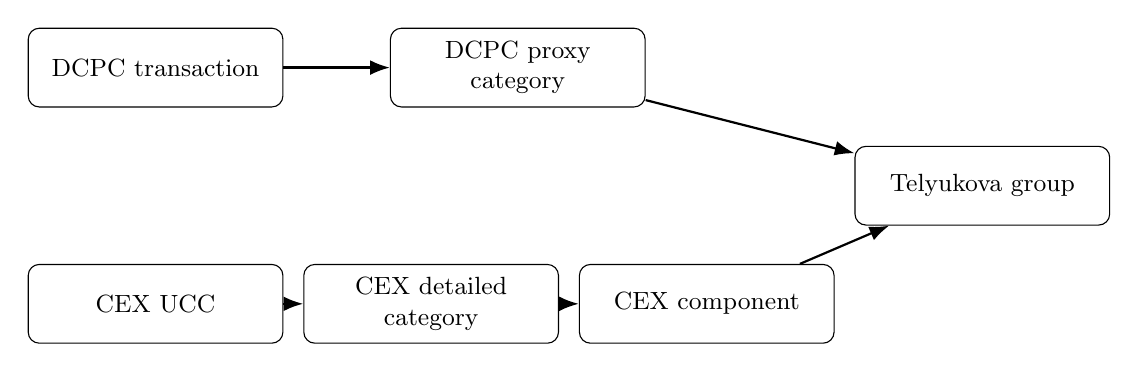
\begin{tikzpicture}[
	box/.style={
		draw,
		rounded corners,
		align=center,
		minimum height=10mm,
		text width=30mm,
		font=\small
	},
	arrow/.style={
		-{Latex[length=2.5mm]},
		thick
	}
	]
	
	% DCPC branch
	\node[box] (dcpc_transaction) at (0,1.5)
	{DCPC transaction};
	
	\node[box] (dcpc_category) at (4.6,1.5)
	{DCPC proxy category};
	
	% CEX branch
	\node[box] (cex_ucc) at (0,-1.5)
	{CEX UCC};
	
	\node[box] (cex_detail) at (3.5,-1.5)
	{CEX detailed category};
	
	\node[box] (cex_component) at (7,-1.5)
	{CEX component};
	
	% Shared aggregation level
	\node[box] (telyukova_group) at (10.5,0)
	{Telyukova group};
	
	% Arrows
	\draw[arrow] (dcpc_transaction) -- (dcpc_category);
	\draw[arrow] (dcpc_category) -- (telyukova_group);
	
	\draw[arrow] (cex_ucc) -- (cex_detail);
	\draw[arrow] (cex_detail) -- (cex_component);
	\draw[arrow] (cex_component) -- (telyukova_group);
	
\end{tikzpicture}

\clearpage

\begin{landscape}
	\footnotesize
	\setlength{\tabcolsep}{5pt}
	\renewcommand{\arraystretch}{1.25}
	
	\begin{longtable}{
			>{\RaggedRight\arraybackslash}p{0.20\linewidth}
			>{\RaggedRight\arraybackslash}p{0.31\linewidth}
			>{\RaggedRight\arraybackslash}p{0.41\linewidth}
		}
		\caption{Identification of DCPC proxy categories}
		\label{tab:dcpc-category-identification}\\
		
		\toprule
		DCPC proxy category &
		Merchant code and meaning &
		Follow-up identification rule and meaning \\
		\midrule
		\endfirsthead
		
		\toprule
		DCPC proxy category &
		Merchant code and meaning &
		Follow-up identification rule and meaning \\
		\midrule
		\endhead
		
		\bottomrule
		\endfoot
		
		\code{food_grocery_proxy} &
		\code{merch}=1: Grocery stores, convenience stores without gas stations,
		and pharmacies. &
		None. The merchant code alone identifies the proxy category. \\
		
		\code{food_restaurant_bar_proxy} &
		\code{merch}=3: Sit-down restaurants and bars. &
		None. The merchant code alone identifies the proxy category. \\
		
		\code{food_fast_service_proxy} &
		\code{merch}=4: Fast-food restaurants, coffee shops, cafeterias, and
		food trucks. &
		None. The merchant code alone identifies the proxy category. \\
		
		\code{rent} &
		\code{merch}=14: Rent for apartments, homes, or other buildings,
		including payments to real-estate companies and property managers. &
		None. The merchant code alone identifies the category. \\
		
		\code{mortgage_payment} &
		\code{merch}=15: Financial-services providers, including mortgage
		companies, banks, credit-card companies, and insurance companies. &
		\code{pay010}=2: Purpose was to make a loan payment; and
		\code{pay011}=1: the loan was a mortgage. \\
		
		\code{utilities} &
		Either \code{merch}=8: Nongovernment utilities, including electricity,
		natural gas, water, sewer, trash, and heating oil; or
		\code{merch}=19: Government taxes or fees. &
		For \code{merch}=8, no follow-up is required.
		
		For \code{merch}=19:
		\code{pay040}=1 means a government purchase of goods or services, and
		\code{pay041}=1 identifies electricity, water, or sewer. \\
		
		\code{communications_entertainment_proxy} &
		\code{merch}=10: Telephone, internet, cable or satellite television,
		streaming services, and movie theaters. &
		None. The merchant code alone identifies the proxy category. \\
		
		\code{household_operations_bill_proxy} &
		\code{merch}=6: General services; or
		\code{merch}=11: Building contractors, plumbers, electricians, and
		HVAC providers. &
		\code{from_bill_section}=1: The transaction originated in the
		bill-reminder section. These records are assigned to household operations
		before the general contractor rule is evaluated. \\
		
		\code{household_repairs} &
		\code{merch}=11: Building contractors, plumbers, electricians, and
		HVAC providers. &
		No additional follow-up. This category contains the remaining
		\code{merch}=11 transactions after the bill-reminder household-operations
		rule has been applied. \\
		
		\code{homeowners_renters_insurance} &
		\code{merch}=15: Financial-services provider. &
		\code{pay010}=3: Purpose was to pay for insurance; and either
		\code{pay016}=1: homeowners insurance, or
		\code{pay016}=2: renters insurance. \\
		
		\code{property_taxes} &
		\code{merch}=19: Government taxes or fees. &
		\code{pay040}=2: Purpose was to pay taxes; and
		\code{pay042}=4: the tax was a property tax. \\
		
		\code{public_transport_tolls} &
		Either \code{merch}=21: Public transportation and tolls; or
		\code{merch}=19: Government taxes or fees. &
		For \code{merch}=21, no follow-up is required.
		
		For \code{merch}=19:
		\code{pay040}=1 means a government purchase of goods or services, and
		either \code{pay041}=5 identifies tolls or
		\code{pay041}=7 identifies public transportation. \\
		
		\code{taxi_air_delivery_proxy} &
		\code{merch}=9: Taxis, airplanes, and delivery services. &
		None. The merchant code alone identifies the proxy category. \\
		
		\code{health_insurance} &
		One of three merchant codes:
		\code{merch}=15, financial services;
		\code{merch}=18, medical-care providers; or
		\code{merch}=19, government. &
		Three alternative rules:
		
		(1) \code{merch}=15, \code{pay010}=3 for insurance, and
		\code{pay016}=3 for health insurance;
		
		(2) \code{merch}=18 and \code{pay030}=4, identifying the payee as an
		insurance company;
		
		(3) \code{merch}=19, \code{pay040}=1 for government goods or services,
		and \code{pay041}=8 for out-of-pocket health insurance, including
		Medicare supplemental insurance. \\
		
		\code{childcare} &
		Either \code{merch}=20: Schools, colleges, and childcare centers; or
		\code{merch}=19: Government taxes or fees. &
		For \code{merch}=20, \code{pay020}=3 identifies childcare.
		
		For \code{merch}=19, \code{pay040}=1 identifies government goods or
		services, and either \code{pay041}=3 identifies daycare or
		\code{pay041}=9 identifies childcare. \\
		
		\code{cash_contributions} &
		\code{merch}=17: Charitable or religious donations. &
		Either \code{pay050}=1: donation; or
		\code{pay050}=2: offering, tithe, or money placed in a collection plate. \\
		
	\end{longtable}
\end{landscape}

\subsection{Estimated Empirical Innovation Volatility}

Table \ref{tab:liquidity-demand-innovation-volatility-2018-2019} reports $\widehat{\alpha}$ and $\operatorname{sd}(\widehat{\eta}_{it})$ from equations (\ref{eqn:telyukova_first_stage}) and (\ref{eqn:telyukova_second_stage}) using monthly CEX data from 2018--2019. The first stage includes calendar-month and calendar-year indicators. Both stages and the reported innovation standard deviations are unweighted. The maintained output files use the legacy column name \lstinline|rho| for $\widehat{\alpha}$; the notation here distinguishes this empirical coefficient from the model persistence $\rho$.

\begin{table}[htbp]
	\centering
	\small
	\setlength{\tabcolsep}{8pt}
	\renewcommand{\arraystretch}{1.2}
	\caption{Monthly empirical innovation-volatility estimates, 2018--2019}
	\label{tab:liquidity-demand-innovation-volatility-2018-2019}
	\begin{tabular}{
			>{\RaggedRight\arraybackslash}p{0.39\textwidth}
			ccc
		}
		\toprule
		Liquid-consumption measure
		& $\widehat{\alpha}$
		& $\operatorname{sd}(\widehat{\eta}_{it})$
		& $\operatorname{sd}(\widehat{\eta}_{it})$ (\%) \\
		\midrule
		Benchmark
		& 0.141 & 0.271 & 27.14 \\
		Excluding food, alcohol, and tobacco
		& 0.139 & 0.285 & 28.53 \\
		Excluding food, alcohol, tobacco, and property taxes
		& 0.109 & 0.325 & 32.47 \\
		\bottomrule
	\end{tabular}
\end{table}

\subsection{Adjacent-Month Liquid-Consumption Correlation for Moment Matching}

The model persistence $\rho$ is calibrated by matching the correlation between liquid consumption in consecutive months. Table \ref{tab:adjacent-consumption-correlations-2019} reports the available 2019 candidate moments in levels and logs. These are pooled, unweighted correlations across strictly consecutive months for which both consumer-unit observations have positive liquid consumption. 

\begin{table}[htbp]
	\centering
	\small
	\setlength{\tabcolsep}{6pt}
	\renewcommand{\arraystretch}{1.2}
	\caption{Adjacent-month liquid-consumption correlations, 2019}
	\label{tab:adjacent-consumption-correlations-2019}
	\resizebox{\textwidth}{!}{%
		\begin{tabular}{
				>{\RaggedRight\arraybackslash}p{0.34\textwidth}
				rrrr
			}
			\toprule
			Liquid-consumption measure
			& Adjacent pairs
			& Consumer units
			& $\operatorname{Corr}(c_{it}^{\mathrm{liq}},c_{i,t-1}^{\mathrm{liq}})$
			& $\operatorname{Corr}(\log c_{it}^{\mathrm{liq}},\log c_{i,t-1}^{\mathrm{liq}})$ \\
			\midrule
			Benchmark
			& 51{,}095 & 11{,}432 & 0.589 & 0.852 \\
			Excluding food, alcohol, and tobacco
			& 50{,}951 & 11{,}397 & 0.560 & 0.844 \\
			Excluding food, alcohol, tobacco, and property taxes
			& 50{,}913 & 11{,}387 & 0.509 & 0.810 \\
			\bottomrule
		\end{tabular}%
	}
\end{table}

\end{document}	
